\documentclass{beamer}

\newcommand{\backupbegin}{
   \newcounter{finalframe}
   \setcounter{finalframe}{\value{framenumber}}
}
\newcommand{\backupend}{
   \setcounter{framenumber}{\value{finalframe}}
}

\usepackage{tikz}
\usepackage[final]{pdfpages}
\usepackage{pgffor}

\setbeamertemplate{navigation symbols}{}


\setbeamercolor{frametitle}{fg=red}
\setbeamercolor{title}{fg=red}

\setbeamerfont{frametitle}{family=\rmfamily,shape=\itshape,size=\huge} 
\setbeamerfont{title}{family=\rmfamily,shape=\itshape,size=\huge} 

\usetheme{boxes}
%\setbeamertemplate{background canvas}[vertical shading][bottom=white,top=blue!20]

\setbeamertemplate{footline}[frame number]

\setbeamertemplate{itemize/enumerate body begin}{\small}
\setbeamertemplate{itemize/enumerate subbody begin}{\footnotesize}

\newcommand{\lyaf}{Lyman-$\alpha$ forest\ }
\newcommand{\lya}{Lyman-$\alpha$\ }
\newcommand{\djc}{{\color{red} !!Jaffe!!}}
\newcommand{\fix}{{\color{red} !!Fix!!}}
\newcommand{\red}[1]{{\color{red}#1}}
\definecolor{orange}{RGB}{255,127,0}
\newcommand{\orange}[1]{{\color{orange}#1}}
\newcommand{\brown}[1]{{\color{brown}#1}}
\newcommand{\blue}[1]{{\color{blue}#1}}


\begin{document}


\begin{frame}
  \frametitle{Overview of LSST  at BNL}

  \begin{center}
    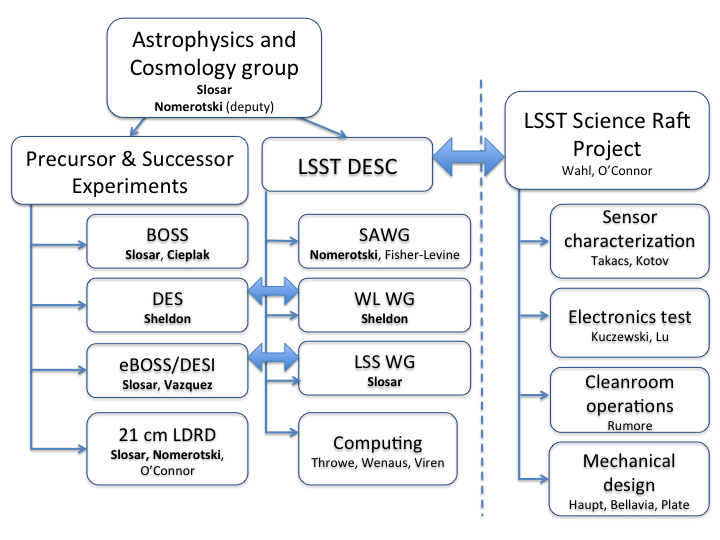
\includegraphics[width=\linewidth]{./chart.png}
  \end{center}
\end{frame}


\begin{frame}
  \frametitle{LSST project at BNL}
  
  In Instrumentation Division:
  \begin{itemize}
  \item At the moment there is \$4.6M  of LSST project funding flowing
    through Instrumentation Division
  \item In total \textbf{25} people, \textbf{14 full time}, 
    excluding Cosmology \& Astrophysics group in Physics
  \item subsystem manager and Physicist for the Camera Science Raft
  \item \textbf{2 FTEs} funded through lab overhead
  \item BNL deliverable: tower raft modules containing focal plane
    sensors and driver / readout electronics
  \item BNL deliverable is performance and schedule critical
  \item \red{\textbf{LSST is a major activity at BNL}}

 \end{itemize}

\end{frame}




\begin{frame}
  \frametitle{BNL's role in LSST DESC}
  
\begin{itemize}

  \item 7 Full Members (Nomerotski,
    May, Sheldon, Slosar, O'Connor, Wenaus, HyeYun Park)

\item Active in
\begin{itemize}
\item Large Scale Structure (Slosar)
\item Sensor Anomalies (Nomerotski)
\item Weak Lensing (Sheldon)
\end{itemize}

\item BNL collaborators helped write large part of Large Scale
  Structure and Sensor Anomalies sections of the \textbf{Science
    Roadmap} (SRM) and its 2017 refactoring

\item BNL collaborators helped with the DESC Science Requirements Document
  
  
 \end{itemize}
\end{frame}

\begin{frame}
  \frametitle{DESC Leadership roles}

  \begin{itemize}
      \item \textbf{Andrei Nomerotski}:
          \begin{itemize}
              \item co-convenor of Sensor Anomalies Working Group
              \item Chair of the DESC Membership committee
              \item member of Collaboration Council
          \end{itemize}

      \item \textbf{Erin Sheldon}:
          \begin{itemize}
              \item WL pipeline Scientists (technical lead)
              \item partly supported on DESC  operations funding
              \item WL working group convenor in DES (LSST precursor)
          \end{itemize}

      \item \textbf{An\v{z}e Slosar}: 
          \begin{itemize}
              \item co-convenor of Large Scale Structure Working Group
              \item member of the LSST Science Advisory Committee (LSST project role)
              \item former member of Collaboration Council, Meetings Committee
              \item helped draft the \emph {DESC Code of Conduct}

        \end{itemize}

    \item \textbf{Tom McClintock}
        \begin{itemize}
            \item Joining BNL as a postdoc in the fall
            \item Leading cosmology with galaxy
                clusters using DC2
        \end{itemize}


\end{itemize}

\end{frame}



\begin{frame}
  \frametitle{University connections re LSST}

  \begin{itemize}


    \item \textbf{Stony Brook}:
      \begin{itemize}
      \item HyeYun Park is a graduate student working in cleanroom and
        DC2 analysis
      \item Anja von der Linden is DESC cluster WG convenor
      \end{itemize}


    \item \textbf{Harvard:}
      \begin{itemize}
      \item Regularly work with Stubbs' group in instrumentation
        issues
      \item collaborated on monocam (see AN talk)
      \end{itemize}

    \item \textbf{Princeton:}
      \begin{itemize}
      \item strong connections on data reduction and management
      \item Former BNL postdoc Fisher-Levine moved to Princeton to
        work on LSST data management
      \end{itemize}
    \item \textbf{Oxford:}
      \begin{itemize}
      \item Will station one postdoc in fall 2018
      \end{itemize}

    \item \textbf{University of Pennsylvania }:
      \begin{itemize}
          \item Sheldon and Jarvis (U. Penn) co-convene the DES Weak Lensing 
              shear pipeline working group and collaborate closely on WL science
      \end{itemize}


\end{itemize}
\end{frame}




\begin{frame}
  \frametitle{LSST DESC Collaboration Meeting 2017 }
  
  \begin{columns}
    \begin{column}{5cm}
      \begin{itemize}
      \item Collaboration meetings hosted at SLAC in the winter and
        participating institutions in the summer
      \item Recognition of the important role BNL plays in the
        collaboration
      \item Meeting was organized together with Stony Brook and was
        deemed a great success

      \end{itemize}
    \end{column}
    \begin{column}{6cm}
      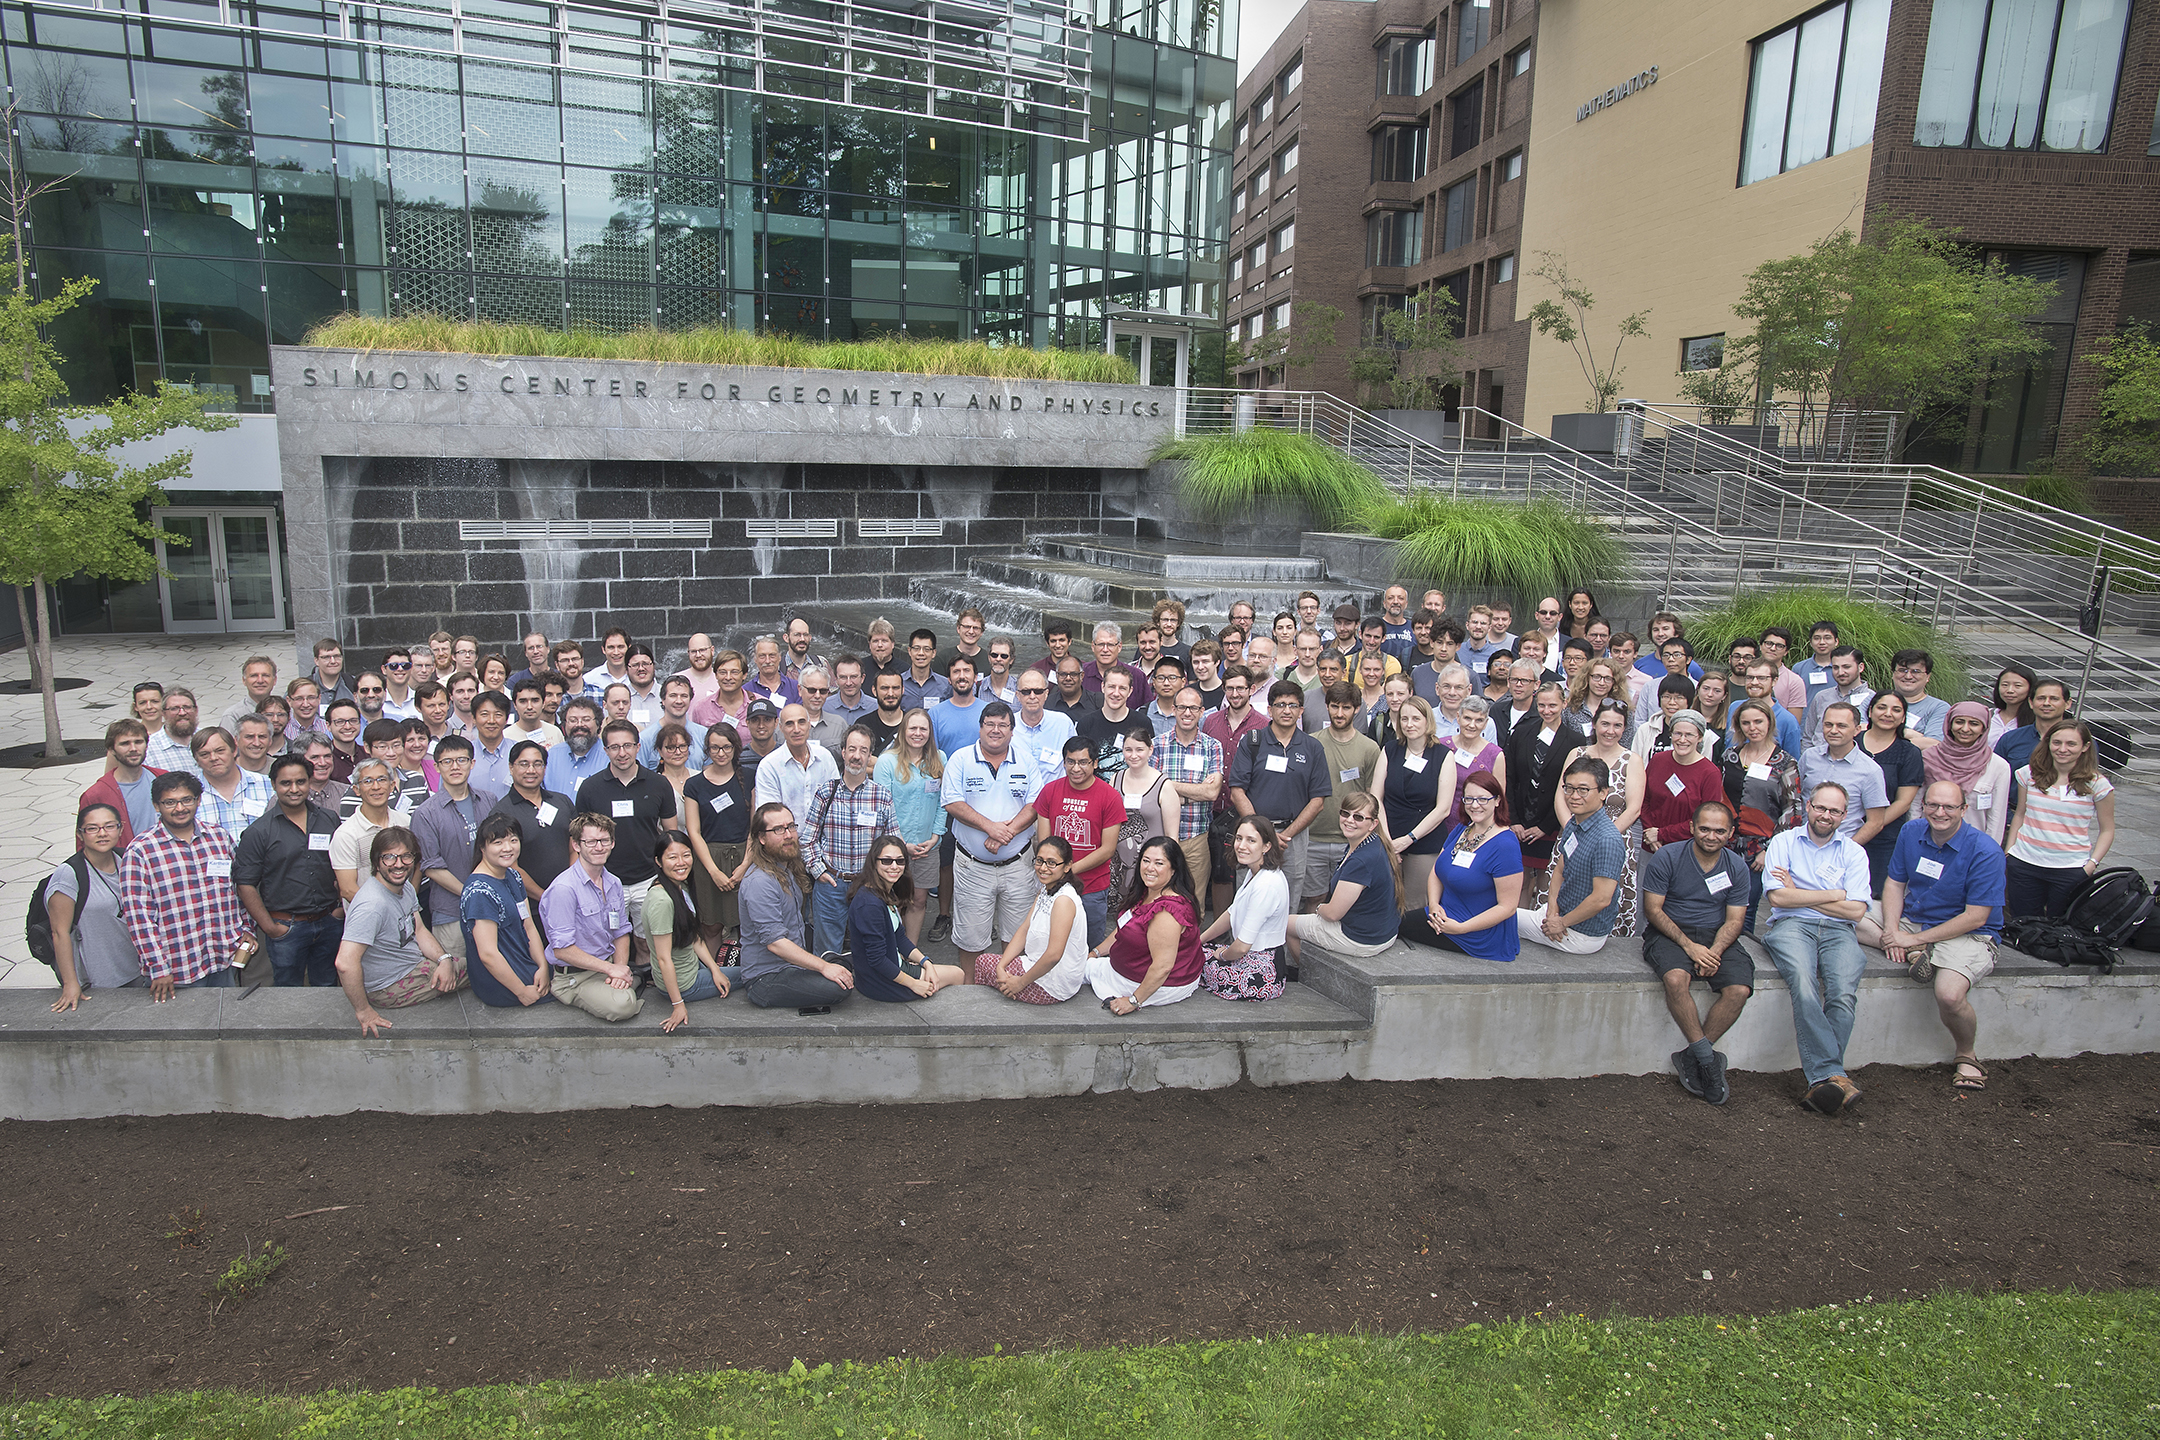
\includegraphics[width=\linewidth]{./D0680717.jpg}
    \end{column}
  \end{columns}


\end{frame}



\begin{frame}
\frametitle {DESC Large Scale Structure WG}

\begin{itemize}  
\item co-chaired by \textbf{Slosar} since January 2016 with David
  Alonso (Oxford)

\item Active in helping develop the 3x2pt pipeline infrastructure and
  novel analysis tools:
  \begin{itemize}
  \item Slosar developed the \texttt{sacc} container class that will
    hold correlations, covariance matrices, etc. for the official
    pipeline

  \item Slosar helped in development of \texttt{NaMaster}, the power
    spectrum estimation tool with capability for full mode projects,
    etc (main developer David Alonso, paper to be ready soon)
  \end{itemize}

\item In addition to infrastructure: four active research projects:

  \begin{itemize}
  \item 2pt-loop: full quick analysis loop for testing
  \item HSC data re-analysis
  \item understanding blending and DM through DC2 input-output catalog
    matching

  \item In conjuction with TJP, we have begun working on project to
  understand modeling beyond linear bias for LSST (co-leading with
  Jonathan Blazek)

  \end{itemize}






\end{itemize}
\end{frame}


\begin{frame}
  \frametitle{2pt validation project}
  
  \begin{columns}
    \begin{column}{8cm}
      \begin{itemize}
        \scriptsize
      \item Lognormal mocks provide a quick short-cut to ``realistic
        enough'' galaxy fields
      \item These fields can be mocked using the full complexity, to
        create toy problems to study systematic effects one by one:
        \begin{itemize}
\scriptsize
        \item photo-z errors
        \item depth fluctuations
        \item stellar contamination
        \item blending
        \item \ldots
        \end{itemize}
      \item In contrast to DCx challenges, we can have O(1000) mocks,
        allowing systematic statistical testing
      \item Basic framework in place
      \end{itemize}




      \vspace*{-0.3cm}
      \begin{center}
      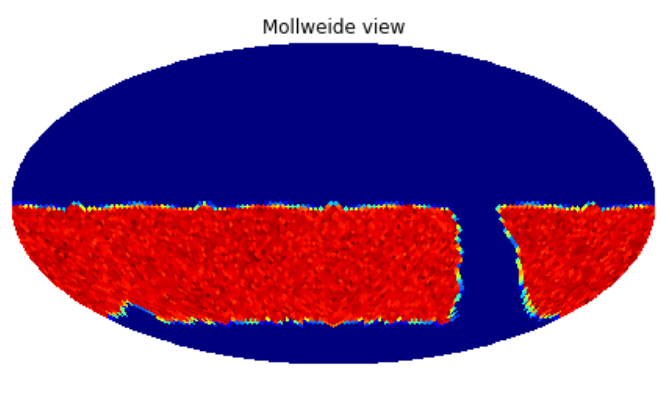
\includegraphics[width=0.45\linewidth]{./random2pt.png}

        \tiny Window function for lognormal mocks based on OpSim runs
      \end{center}



    \end{column}
    \begin{column}{4cm}
      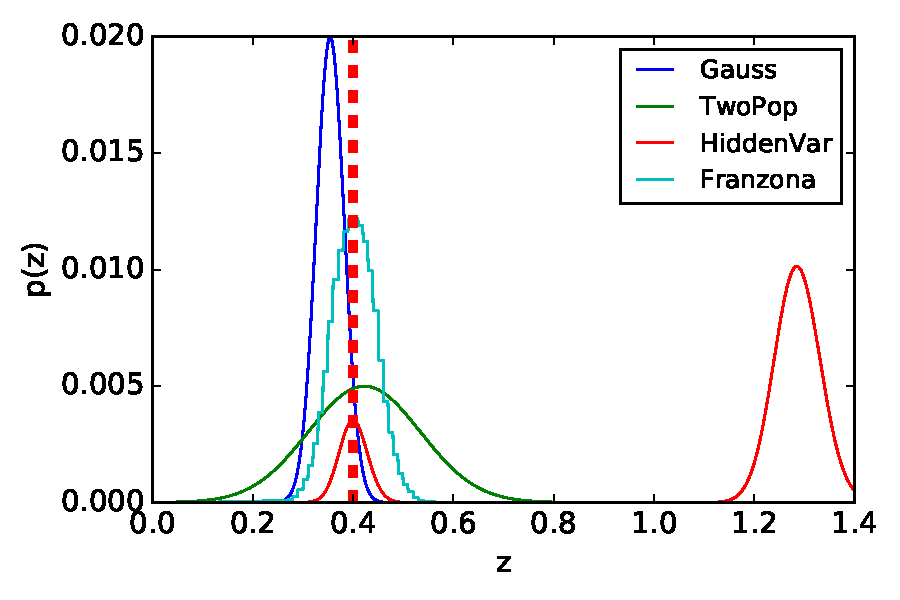
\includegraphics[width=\linewidth]{./ptest04.pdf}
      \vspace*{-0.3cm}
      \begin{center}
        \tiny Different photo-z models developed for 2-pt validation
      \end{center}

      \begin{center}
        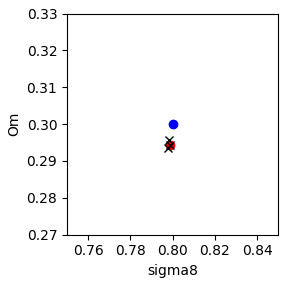
\includegraphics[width=0.8\linewidth]{./xx.png}

        \tiny First full round-trip recovering the input $\Omega_M$
        and $\sigma_8$ with small, but non-negligible biases

      \end{center}
    \end{column}
  \end{columns}
\end{frame}


\begin{frame}
  \frametitle{HSC reanalysis}

  \begin{columns}
    \begin{column}{5cm}
      \begin{itemize}
      \item Idea is to test the LSST pipeline tools on HSC data
      \item HSC data analyses with the same code as LSST
      \item Tools not quite ready, but trying to use them makes all
        the deficiencies obvious
      \item Goal is to measure power-spectrum of galaxy clustering and
        characterise bias evolution of likely LSST source
      \item Stretch goal is to detect magnification
      \end{itemize}
    \end{column}
    \begin{column}{6cm}
      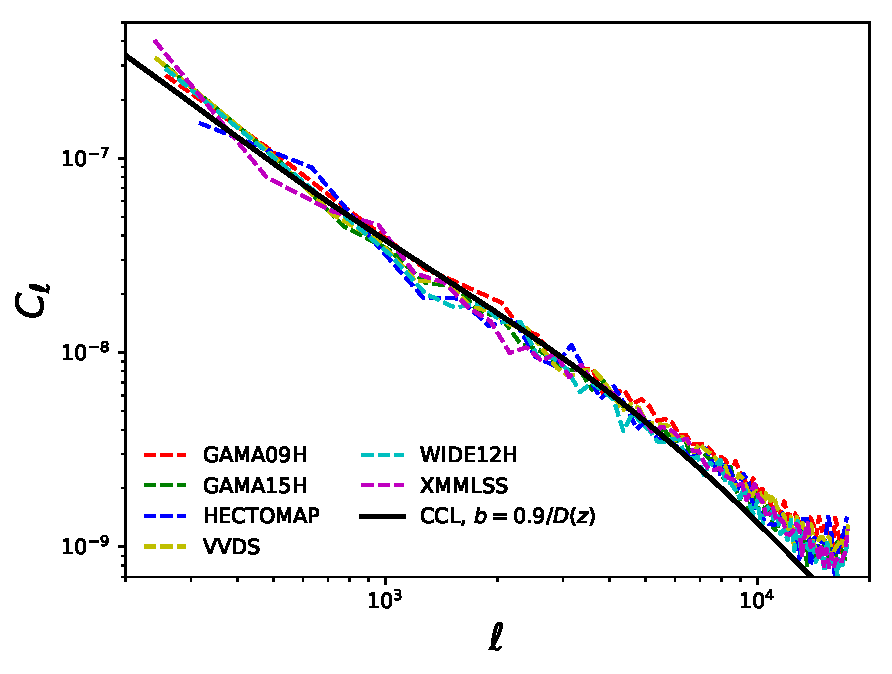
\includegraphics[width=\linewidth]{./cls_hsc.pdf}
      \begin{center}
        \scriptsize Preliminary re-analysis of HSC data. Measured
        power-spectrum consistent across fields 
      \end{center}

    \end{column}
  \end{columns}


\end{frame}


\begin{frame}
  \frametitle{DC2 matching}

  \begin{columns}
    \begin{column}{7.5cm}
      \begin{itemize}
      \item Connecting input and output catalogs is non-trivial
      
      \item We want to do matching with minimal assumptions and
        flagging in order to \emph{study} what various flags do

      \item Using a novel Friends-of-friends based algorithm to
        preselect data into:
        \begin{itemize}
          \scriptsize
        \item  pure false positives (detections where
        there is nothing around in the input catalog)

      \item pure non-detections (input catalog objects without any
         detections in the output catalog)

      \item clear 1-1 matches (there is one input object and one
        output object and nothing else in the area)

      \item everything else (actual blends, wrongly identified blends,
        failed deblends, etc.)


        \end{itemize}
      \item Preliminary results very encouraging, numerous
        possibilities for true understanding of data reduction

      \end{itemize}
    \end{column}
    \begin{column}{5cm}
      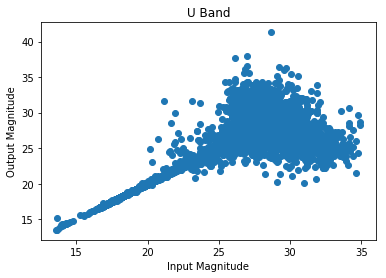
\includegraphics[width=\linewidth]{./image.png}
      \begin{center}
\scriptsize
        Input vs Output $u$-band magnitude for sources that are unique
        1-1 pairs within arcsec and are closer than 0.1 arcsec in separation
        {\color{red}{AS: to be fixed}}
      \end{center}
    \end{column}
  \end{columns}



\end{frame}


\frame
{

    \frametitle{Weak Lensing Pipeline Scientist}

    \begin{columns}
        \begin{column}{0.7\textwidth}


            \begin{itemize}

                \item Erin Sheldon is a DESC 
                    pipeline scientist working on weak lensing
                    shear catalogs.

                \item Responsible for creating software 
                    pipelines to measure weak lensing shear.

                \item Responsible for producing, or coordinating
                    the production, of the shear catalogs.

                \item Adapting codes from the Dark
                    Energy Survey (metacalibration, MEDS,
                    the MOF deblender, etc.)

                \item Current focus is on reprocessing the HSC survey
                    and processing the DESC data challenge 2 (DC2)

            \end{itemize}


        \end{column}

        \begin{column}{0.3\textwidth}
            \begin{center}
                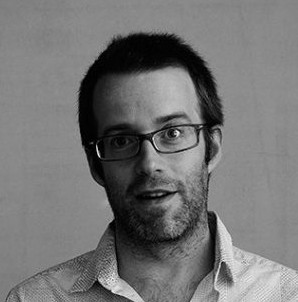
\includegraphics[width=\textwidth]{sheldon.png}
                %
\includegraphics[width=\textwidth]{TomMportrait.jpg}
                %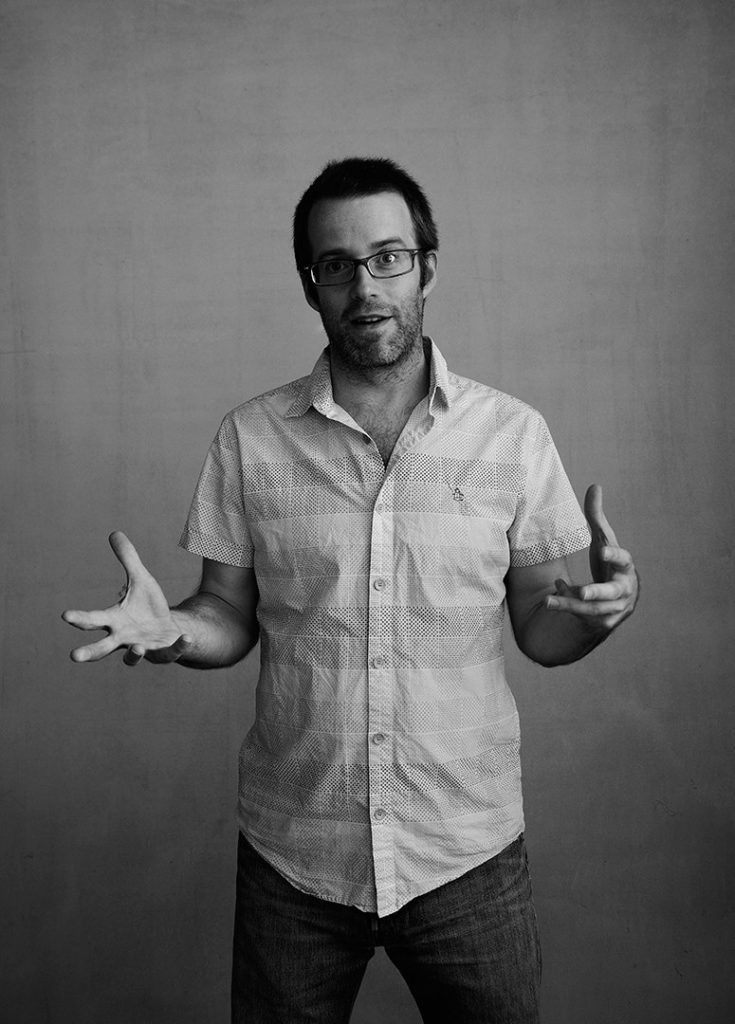
\includegraphics[width=\textwidth]{erin-sheldon-735x1024.jpg}
                \newline
                {\tiny Erin Sheldon}
            \end{center}
        \end{column}

    \end{columns}

}

\frame
{

    \frametitle{Weak Lensing Pipeline Scientist: Progress}

    %\setbeamerfont*{itemize/enumerate body}{size=\large}

    \begin{itemize}

        \item Sheldon has produced the framework to
            use the LSST data interface (the Butler) to
            produce the inputs needed for the shear
            pipelines.

        \item The shear code has been run on the inputs, 
            and catalogs produced, for a subset of the 
            HSC data.  This is all the data that
            was available at the time.

        \item The code is ready to run on the full HSC
            and DC2 when available.

    \end{itemize}
}

\frame
{

    \frametitle{Weak Lensing Pipeline Scientist: Future}

    %\setbeamerfont*{itemize/enumerate body}{size=\large}

    \begin{itemize}

        \item Working with Francois Lanusse (CMU) to get the processing
            of DC2 working at NERSC. Francois plans to take on the
            actual production.

        \item Help the working group to test and use the outputs.

        \item A new HSC reprocessing should be available soon, and
            shear catalogs will be produced.  This could 
            potentially lead to science papers.

        \item Get other DES codes working as well: MOF Image Deblender

        \item Help to prepare other codes, e.g. BFD (Bernstein et al.)

        \item Get some of the interface code worked into LSST DM

    \end{itemize}
}

\frame
{

    \frametitle{Cluster Cosmology with LSST}

    %\setbeamerfont*{itemize/enumerate body}{size=\large}

    \begin{columns}
        \begin{column}{0.5\textwidth}

            \begin{itemize}

                \item Tom McClintock will be joining BNL as a postdoc
                    in Fall 2018.

                \item Tom is the DC2 cluster cosmology project lead.

                \item Leading the the inference of cosmological parameters
                    using cluster lensing.

                \item Tom lead a similar analysis of DES year 1 data, so
                    he is eminently qualified.

            \end{itemize}
        \end{column}

        \begin{column}{0.5\textwidth}
            \begin{center}
                
\includegraphics[width=\textwidth]{TomMportrait.jpg}
                \newline
                {\tiny Tom McClintock}
            \end{center}
        \end{column}

    \end{columns}


}







\end{document}
